% \documentclass{ijsra}
\def\IJSRAidentifier{\currfilebase} %<---- don’t change this!
\def\submission{}%YYYY-MM-DD
\def\acceptance{}%YYYY-MM-DD
%-------Title | Email | Keywords | Abstract-------------
\def\shorttitle{The Economy of Pre-Colonial Zimbabwe}
\def\maintitle{Intracontinental Exchanges Before \enquote{Globalization}: The Economy of Pre-Colonial Zimbabwe}
% \footnote{Paper presented at ICAHM 2017 Annual Conference held in Bagamoyo, Tanzania from 2-5 October.}
\def\cmail{humphreynyambiya@gmail.com}
\def\keywords{trade, globalization, pre-colonial Zimbabwe, Great Zimbabwe, Mutapa State, Rozvi State}
%\def\keywordname{}%<--- redefine the name “Keywords“ in needed language
\def\abstract{Paper presented at ICAHM 2017 Annual Conference held in Bagamoyo, Tanzania from 2-5 October.


Globalization and capitalism, which structures current modes of relationships are often traced to the European conquest and colonization of the global south. But long-distance trade, industrialization, and mass consumption have their roots in early interactions. These interactions were often local and regional in scope which however increased in complexity and scale. A focus on long-distance exchange as a prime factor in the rise of socially complex chiefdoms and states has often overlooked regional economic networks upon which later economic and cultural interactions interlocked
\parencite{kusimba2017}.
Based on the review of literature available on trade, this paper argues that regional and interregional trade involving pre-colonial Zimbabwe were forms of globalization which predate international contacts. This paper evaluates the impact of regional and interregional trade to the economies of pre-colonial Zimbabwean societies particularly Great Zimbabwe, Mutapa, and the Rozvi states. A discussion of the contribution of this branch of the economy (regional and interregional trade) to international trade is also presented. Given the nature of the available literature on regional and interregional trade involving pre-colonial Zimbabwe, the paper finally proposes a multi-disciplinary approach to the understanding of this system of trade.}
%--------Author’s names------------
\def\authorone{Humphrey Nyambiya}
%-------Biographical information-------------
\def\bioone{Humphrey Nyambiya is a (BA Hons) student in Archaeology at the University of Zimbabwe. His research interests are ancient trade and trade routes, geoarchaeology, and environmental archaeology. He is also interested in heritage management, sustainable development, and community participation in heritage management.}
%------University/Institution--------------
\def\affilone{University of Zimbabwe}
\iffalse
\begin{filecontents}{\IJSRAidentifier.bib}
@article{ab1961,
	author  = "Abraham, D.P.",
	title   = "Maramuca: An exercise in the combined use of Portuguese records and oral tradition",
	journal = "The Journal of African History",
	year    = "1961",
	volume  = "2",
	number  = "2",
	pages   = "211-225"
}
@article{ashley2015,
	author  = "Ashley, C.Z. and K.M. Grillo",
	title   = "Archeological ceramics from eastern Africa: Past approaches and future directions",
	journal = "Azania: Archaeological Research in Africa",
	year    = "2015",
	volume  = "50",
	number  = "4",
	pages   = "460-480"
}
@article{baron2014,
	author  = "Baron, S. and C.G. Tamas and C. Le Carlier",
	title   = "How mineralogy and geochemistry can improve the significance of Pb isotopes in metal provenance studies",
	journal = "Archaeometry",
	year    = "2014",
	volume  = "56",
	number  = "4",
	pages   = "665-680"
}
@article{beach1976,
	author  = "Beach, D.N.",
	title   = "The Mutapa dynasty: A comparison of documentary and traditional evidence",
	journal = "History in Africa",
	year    = "1976",
	volume  = "3",
	pages   = "1-17"
}
@book{beach1980,
	author    = "D.N. Beach",
	title     = "The Shona and Zimbabwe, 900--1850: An Outline of Shona History",
	publisher = "Mambo Press",
	year      = "1980",
	address   = "Gweru"
}
@article{beach1998,
	author  = "Beach, D.N.",
	title   = "Cognitive archaeology and imaginary history at Great Zimbabwe",
	journal = "Current Archaeology",
	year    = "1998",
	volume  = "39",
	number  = "1",
	pages   = "47-72"
}
@article{bvocho2005,
	author  = "Bvocho, G.",
	title   = "Ornaments as social and chronological icons: A case study of south-eastern Zimbabwe",
	journal = "Journal of Social Archaeology",
	year    = "2005",
	volume  = "5",
	number  = "3",
	pages   = "409-424"
}
@article{chanaiwa1972,
	author  = "Chanaiwa, D.",
	title   = "Politica and long-distance trade in the Mwene Mutapa Empire during the sixteenth century",
	journal = "The International Journal of African Hisrorical Studies",
	year    = "1972",
	volume  = "5",
	number  = "3",
	pages   = "424-435"
}
@article{chirikure2008,
	author  = "Chirikure, S. and I. Pikirayi",
	title   = "Inside and outside the dry stone walls: revisiting material culture of Great Zimbabwe",
	journal = "Antiquity",
	year    = "2008",
	volume  = "82",
	pages   = "976-993"
}
@phdthesis{chirikure2005,
	author = "Chirikure, S.",
	title  = "Iron Production in Iron Age Zimbabwe: Stagnation or Innovation?",
	school = "University College London",
	year   = "2005"
}
@article{chirikure2006,
	author  = "Chirikure, S.",
	title   = "New light on Njanja iron working: Towards a systematic encounter between ethnohistory and archaeometallurgy",
	journal = "South African Archaeological Bulletin",
	year    = "2006",
	volume  = "61",
	number  = "184",
	pages   = "142-151"
}
@article{chirikure2007,
	author  = "Chirikure, S.",
	title   = "Metals in society: Iron production and its position in Iron Age communities of southern Africa",
	journal = "Journal of Social Archaeology",
	year    = "2007",
	volume  = "7",
	number  = "1",
	pages   = "72-100"
}
@book{chirikure2010,
	author    = "Chirikure, S.",
	title     = "Indigenous mining and metallurgy in Africa",
	publisher = "Cambridge University Press",
	year      = "2010",
	address   = "Cambridge"
}
@book{chirikure2015,
	author    = "Chirikure, S.",
	title     = "Metals in Past Societies: A Global Perspective on Indigenous African Metallurgy",
	publisher = "Springer",
	year      = "2015",
	address   = "New York"
}
@article{chirikure2013socio,
	author  = "Chirikure, S. and M. Manyanga and A.M. Pollard and I. Pikirayi",
	title   = "New pathways of sociopolitical complexity in southern Africa",
	journal = "African Archaeological Review",
	year    = "2013",
	volume  = "30",
	number  = "4",
	pages   = "339-366"
}
@incollection{chirikure2013post,
	author    = "Chirikure, S. and  T.P. Thondhlana and F. Bandama",
	booktitle = "Zimbabwean archaeology in the Post-Independence era",
	editor    = "Manyanga, M.  and Katsamudanga, S.",
	title     = "Pre-colonial mining and metalworking in southern Africa: An overview with specific reference to Zimbabwe",
	publisher = "Sapes Books",
	year      = "2013"
}
@article{chirikure2014,
	author  = "Chirikure, S. and M. Manyanga and A.M. Pollard and F. Bandama and G. Mahachi and I. Pikirayi",
	title   = "Zimbabwe Culture before Mapungubwe: New Evidence from Mapela Hill, South-Western Zimbabwe",
	journal = "PLoS ONE",
	year    = "2014",
	volume  = "9",
	number  = "10",
	pages   = "1-18"
}
@article{chirikure2017,
	author  = "Chirikure, S. and  T. Moultrie and F. Bandama and C. Dandara and M. Manyanga",
	title   = "What was the population of Great Zimbabwe (CE1000-1800)?",
	journal = "PLoS ONE",
	year    = "2017",
	volume  = "12",
	number  = "6"
}
@phdthesis{chiripanhura2017,
	author = "Chiripanhura, P.",
	title  = "Archaeological Collections As A Prime Research Asset: Objects And Great Zimbabwe’s Past",
	school = "University of Cape Town",
	year   = "2017"
}
@article{dussubieux2008,
	author  = "Dussubieux, L. and C.M. Kusimba and V. Gogte and S.B. Kusimba and B. Gratuze and R. Oka",
	title   = "The trading of ancient glass beads: new analytical data from South Asian and East African soda-alumina glass beads",
	journal = "Archaeometry",
	year    = "2008",
	volume  = "50",
	number  = "5",
	pages   = "797-821"
}
@article{garlake1968,
	author  = "Garlake, P.S.",
	title   = "The Value of Imported Ceramics in the Dating and Interpretation of the Rhodesian Iron Age",
	journal = "The Journal of African History",
	year    = "1968",
	volume  = "9",
	number  = "1",
	pages   = "13-33"
}
@book{garlake1973,
	author    = "Garlake, P.S.",
	title     = "Great Zimbabwe",
	publisher = "Thames and Hudson",
	year      = "1973",
	address   = "London"
}
@book{garlake1982,
	author    = "Garlake, P.S.",
	title     = "Great Zimbabwe Described and Explained",
	publisher = "Zimbabwe Publishing House",
	year      = "1982",
	address   = "Harare"
}
@book{hall1990,
	author    = "Hall, M.",
	title     = "Farmers, kings and traders: The peoples of southern Africa, 200--1860",
	publisher = "University of Chicago Press",
	year      = "1990",
	address   = "Chicago"
}
@article{huffman2011,
	author  = "Huffman, T.N. and J. Du Piesanie",
	title   = "Khami and the Venda in the Mapungubwe Landscape",
	journal = "Journal of African Archaeology",
	year    = "2011",
	volume  = "9",
	number  = "2",
	pages   = "189-206"
}
@article{huffman1972,
	author  = "Huffman, T.N.",
	title   = "The rise and fall of Zimbabwe",
	journal = "The Journal of African History",
	year    = "1972",
	volume  = "13",
	number  = "3",
	pages   = "353-366"
}
@article{huffman1982,
	author  = "Huffman, T.N.",
	title   = "Archaeology and ethnohistory of the African Iron Age",
	journal = "Annual Review of Anthropology",
	year    = "1982",
	volume  = "11",
	pages   = "133-150"
}
@incollection{huffman1984b,
	author    = "Huffman, T.N.",
	booktitle = "Frontiers: Southern African archaeology today",
	editor    = "Hall, M. and Avery, G. and Avery, D.M. and Wilson, M.L. and Humphreys, A.J.B.",
	title     = "Where you are the girls gather to play: The Great Enclosure at Great Zimbabwe",
	publisher = "British Archaeological Reports (Oxford) Ltd",
	year      = "1984",
	address   = "Cambridge"
}
@article{huffman1984a,
	author  = "Huffman, T.N.",
	title   = "Expressive space in the Zimbabwe Culture",
	journal = "Man",
	year    = "1984",
	volume  = "19",
	number  = "4",
	pages   = "593-612"
}
@article{huffman1986,
	author  = "Huffman, T.N.",
	title   = "Cognitive studies of the iron age in southern Africa",
	journal = "World Archaeology",
	year    = "1986",
	volume  = "18",
	number  = "1",
	pages   = "84-95"
}
@book{huffman1996,
	author    = "Huffman, T.N.",
	title     = "Snakes and crocodiles: power and symbolism in ancient Zimbabwe",
	publisher = "Witwatersrand University Press",
	year      = "1996",
	address   = "Johannesburg"
}
@article{huffman2000,
	author  = "Huffman, T.N.",
	title   = "Mapungubwe and the origins of the Zimbabwe culture",
	journal = "South African Archaeological Society",
	year    = "2000",
	volume  = "8",
	pages   = "14-21"
}
@article{huffman2009,
	author  = "Huffman, T.N.",
	title   = "Mapungubwe and Great Zimbabwe: The origin and spread of social complexity in southern Africa",
	journal = "Journal of Anthropological Archaeology",
	year    = "2009",
	volume  = "28",
	pages   = "37-54"
}
@article{huffman2010,
	author  = "Huffman, T.N.",
	title   = "Revisiting Great Zimbabwe",
	journal = "Azania: Archaeological research in Africa",
	year    = "2010",
	volume  = "45(3)",
	pages   = "321-328"
}
@article{huffman2012,
	author  = "Huffman, T.N.",
	title   = "Historical archaeology of the Mapungubwe area: Boer, Birwa, Sotho-Tswana and Machete",
	journal = "Southern African Humanities",
	year    = "2012",
	volume  = "24",
	pages   = "33-59"
}
@article{huffman2014,
	author  = "Huffman, T.N.",
	title   = "Ritual space in the Zimbabwe Culture",
	journal = "Ethnoarchaeology",
	year    = "2014",
	volume  = "6",
	number  = "1",
	pages   = "4-39"
}
@article{huffman2015,
	author  = "Huffman, T.N.",
	title   = "Social Complexity in Southern Africa",
	journal = "African Archaeological Review",
	year    = "2015",
	volume  = "32",
	number  = "1",
	pages   = "71-91"
}
@article{kim2008,
	author  = "Kim, N.C. and C.M. Kusimba",
	title   = "Pathways to Social Complexity and State Formation in the Southern Zambezian Region",
	journal = "African Archaeological Review",
	year    = "2008",
	volume  = "25",
	pages   = "131-152"
}
@phdthesis{kinahan2000,
	author = "Kinahan, J.",
	title  = "Cattle for Beads: the historical contact and trade on the Namid Coast",
	school = "Uppsala University",
	year   = "2000"
}
@book{kusimba1999,
	author    = "Kusimba, C.M.",
	title     = "The rise and fall of Swahili states",
	publisher = "AltaMira",
	year      = "1999",
	address   = "Walnut Creek"
}
@incollection{kusimba2007,
	author    = "Kusimba, C.M.",
	booktitle = "Archaeology of Atlantic Africa and the African Diaspora",
	editor    = "Ogundiran, A. and T. Falola",
	title     = "The collapse of coastal city-states of East Africa",
	publisher = "Indiana University Press",
	year      = "2007",
	address   = "Bloomington",
	note      = "160-184"
}
@incollection{kusimba2017,
	author    = "Kusimba, C.M. and N.C. Kim and S. Kusimba",
	booktitle = "Feast, Famine or Fighting?: Multiple pathways to social complexity. Studies in human ecology and adaptation",
	editor    = "Chacon, R.J. and Mendoza, R.G.",
	title     = "Trade and state formation in ancient east African coast and southern Zambezia",
	publisher = "Springer International Publishing AG",
	year      = "2017",
	address   = "Cham",
	note      = "61-89"
}
@article{lindahl2010,
	author  = "Lindahl, A. and I. Pikirayi",
	title   = "Ceramics and change: an overview of pottery production techniques in northern South Africa and eastern Zimbabwe during the first and second millennium AD",
	journal = "Archaeological and Anthropological Sciences",
	year    = "2010",
	volume  = "2",
	number  = "3",
	pages   = "133-149"
}
@phdthesis{manyanga2006,
	author = "Manyanga, M.",
	title  = "Resilient landscapes: socio-environmental dynamics in the Shashi-Limpopo Basin, southern Zimbabwe c. AD 800 to the present",
	school = "Uppsala University",
	year   = "2006"
}
@incollection{manyanga2010,
	author    = "Manyanga, M. and I. Pikirayi and S. Chirikure",
	booktitle = "The urban mind: Cultural and environmental dynamics",
	editor    = "Sinclair, P.J.J. and  Nordquist, G. and Herschend, F.  and Isendahl, C.",
	title     = "Conceptualising the urban mind in Pre-European southern Africa: Rethinking Mapungubwe and Great Zimbabwe",
	publisher = "Uppsala University",
	year      = "2010",
	note      = "573-590"
}
@article{miller2000,
	author  = "Miller, D. and N. Desai and J. Lee-Thorp",
	title   = "Indigenous Gold Mining in Southern Africa: A Review",
	journal = "South African Archaeological Society Goodwin Series",
	year    = "2000",
	volume  = "8",
	pages   = "91-99"
}
@book{mitchell2002,
	author    = "Mitchell, P.",
	title     = "The archaeology of southern Africa",
	publisher = "Cambridge University Press",
	year      = "2002",
	address   = "Cambridge"
}
@mastersthesis{molofsky2009,
	author = "Molofsky, J.L.",
	title  = "A Novel Approach To Lead Isotope Provenance Studies Of Tin And Bronze",
	school = "University of Arizona",
	year   = "2009"
}
@article{mudenge1974,
	author  = "Mudenge, S.I.",
	title   = "The role of foreign trade in the Rozvi Empire: A reappraisal",
	journal = "The Journal of African History",
	year    = "1974",
	volume  = "XV",
	number  = "3",
	pages   = "373-391"
}
@book{mudenge1988,
	author    = "Mudenge, S.I.",
	title     = "A Political History of Munhumutapa",
	publisher = "Zimbabwe Publishing House",
	year      = "1988",
	address   = "Harare"
}
@article{ndoro1997,
	author  = "Ndoro, W.",
	title   = "Great Zimbabwe",
	journal = "Scientific American",
	year    = "1997",
	pages   = "94-99",
}
@phdthesis{ndoro2001,
	author = "Ndoro, W.",
	title  = "Your monument our shrine: The preservation of Great Zimbabwe",
	school = "Uppsala University",
	year   = "2001",
}
@incollection{pernicka2014,
	author    = "Pernicka, E.",
	booktitle = "Archaeometallurgy in global perspective",
	editor    = "Roberts, B. W. and Thornton, C.P.",
	pages     = "239-268",
	publisher = "Springer",
	title     = "Provenance determination of archaeological metal objects",
	year      = "2014",
	address   = "New York",
}
@article{pikirayi2011,
	author    = "Pikirayi, I. and S. Chirikure",
	title     = "Debating Great Zimbabwe",
	journal   = "Azania: Archaeological Research in Africa",
	year      = "2011",
	volume    = "46",
	number    = "2",
	pages     = "221-231",
}

@article{pikirayi2009,
	author    = "Pikirayi, I.",
	title     = "Palaces, feiras and prazos",
	subtitle = {An historical archaeological perspective of African–Portuguese contact in Northern Zimbabwe},
	journal   = "African Archaeological Review",
	year      = "2009",
	volume    = "26",
	pages     = "163--185",
}

@phdthesis{pikirayi1993,
	author    = "Pikirayi, I.",
	title     = "The archaeological identity of the Mutapa state: towards an historical archaeology of northern Zimbabwe",
	school    = "Uppsala University",
	year      = "1993",
}
@incollection{pikirayi1996,
	author    = "Pikirayi, I.",
	booktitle = "Aspects of African archaeology: Papers from the 10th Congress of the PanAfrican Association for prehistory and related studies",
	editor    = "Pwiti, G. and Soper, R.",
	title     = "Ceramics and culture change in northern Zimbabwe: on the origins of the Musengezi tradition",
	publisher = "University of Zimbabwe Publications",
	year      = "1996",
	address   = "Harare",
	pages     = "629-639"
}
@book{pikirayi2001,
	author    = "Pikirayi, I.",
	title     = "The Zimbabwe Culture: Origins and Decline of Southern Zambezian States",
	publisher = "AltaMira",
	year      = "2001",
	address   = "Walnut Creek"
}
@incollection{pikirayi2006,
	author    = "Pikirayi, I.",
	booktitle = "Cities in the World, 1500--2000: papers given at the conference of the Society for Post-Medieval Archaeology",
	editor    = "Green, A. and R. Leech",
	title     = "The demise of Great Zimbabwe, AD 1420--1550: an environmental re-appraisal",
	publisher = "Maney",
	year      = "2006",
	address   = "Leeds",
	note      = "31-47"
}
@article{pikirayi2007,
	author  = "Pikirayi, I.",
	title   = "Ceramics and group identities: Towards a social archaeology in southern African Iron Age ceramic studies",
	journal = "Journal of Social Archaeology",
	year    = "2007",
	volume  = "7",
	pages   = "286-301"
}
@article{pikirayi2013archit,
	author  = "Pikirayi, I.",
	title   = "Stone architecture and the development of power in the Zimbabwe Tradition A.D 1270-1830",
	journal = "Azania: Archaeological Research in Africa",
	year    = "2013",
	volume  = "48",
	number  = "2",
	pages   = "282-300"
}
@article{pikirayi2013hist,
	author  = "Pikirayi, I.",
	title   = "Great Zimbabwe in Historical Archaeology: Reconceptualizing Decline, Abandonment, and Reoccupation of an Ancient Polity, A.D. 1450-1900",
	journal = "Historical Archaeology",
	year    = "2013",
	volume  = "47",
	number  = "1",
	pages   = "26-37"
}
@article{pikirayi2017,
	author  = "Pikirayi, I.",
	title   = "Trade, globalisation and the archaic state in southern Africa",
	journal = "Journal of Southern African Studies",
	year    = "2017",
	pages   = "1-15"
}
@article{pwiti1991,
	author  = "Pwiti, G.",
	title   = "Trade and economies in southern Africa: the archaeological evidence",
	journal = "Zambezia",
	year    = "1991",
	volume  = "XVIII",
	number  = "II",
	pages   = "119-129"
}
@phdthesis{pwiti1996,
	author = "Pwiti, G.",
	title  = "Continuity and change: An archaeological study of farming communities in northern Zimbabwe AD 500-1700",
	school = "Uppsala University",
	year   = "1996"
}
@incollection{pwiti2005,
	author    = "Pwiti, G.",
	booktitle = "African archaeology: a critical introduction",
	editor    = "Stahl, A.B.",
	title     = "Southern Africa and the East African Coast",
	publisher = "Blackwell Publishing",
	year      = "2005",
	address   = "Oxford",
	note      = "378-391"
}
@book{randall1906,
	author    = "Randall-MacIver, D.",
	title     = "Mediaeval Rhodesia",
	publisher = "Macmillan",
	year      = "1906",
	address   = "London"
}
@article{robertshaw2010,
	author  = "Robertshaw, P. and  M. Wood and  E. Melchiorre and  R.S. Popelka-Filcoff and M.D. Glascock",
	title   = "Southern African glass beads: Chemistry, glass sources and patterns of trade",
	journal = "Journal of Archaeological Science",
	year    = "2010",
	volume  = "37",
	pages   = "1898-1912"
}
@incollection{alradi1990,
	author    = "al-Radi, S.",
	title     = "The architecture of housing: exploring architecture in Islamic cultures",
	editor    = "Powell, R.",
	title     = "A brief history of the east African coast",
	publisher = "Aga Khan Award for architecture",
	year      = "1990",
	note      = "270-276"
}
@incollection{sinclair1993,
	author    = "Sinclair, P.J.J. and  I. Pikirayi and G. Pwiti and R. Soper",
	booktitle = "The archaeology of Africa: Food, metals and towns",
	editor    = "Shaw, T. and P.J.J. Sinclair and B. Andah and A. Okpoko",
	title     = "Urban trajectories on the Zimbabwe plateua",
	publisher = "Routledge",
	year      = "1993",
	address   = "London",
	pages     = "705-731"
}
@article{tangri1990,
	author  = "Tangri, D.",
	title   = "Popular fiction and the Zimbabwe controversy",
	journal = "History in Africa",
	year    = "1990",
	volume  = "17",
	pages   = "293-304"
}
@article{wilmsen2009,
	author  = "Wilmsen, E.N. and D. Killick and D.D. Rosenstein and P.C. Thebe and J.R. Denbow",
	title   = "The social geography of pottery in Botswana as reconstructed by optical petrography",
	journal = "Journal of African Archaeology",
	year    = "2009",
	volume  = "7",
	number  = "1",
	pages   = "3-39",
}
@article{wood2000,
	author  = "Wood, M.",
	title   = "Making Connections: Relationships between international trade and glass beads from the Shashe-Limpopo area",
	journal = "South African Archaeological Society Goodwin Series",
	year    = "2000",
	volume  = "8",
	pages   = "78-90"
}
@book{sinclair1987,
	author    = "Sinclair, P.J.J.",
	title     = "Space, Time and Social Formation: A Territorial Approach to the Archaeology and Anthropology of Zimbabwe and Mozambique, c. 0--1700 A.D.",
	publisher = "Societas Archaeologica Upsaliensis",
	year      = "1987",
	address   = "Uppsala"
}
\end{filecontents}
\fi
\IJSRAopening%<---- don’t change this!
%-------

\IJSRAsection{Introduction}
\begin{IJSRAquote}{\cite[6]{pikirayi2017}}
% \blockcquote[6]{pikirayi2017}
{The role of regional and intercontinental exchange remains very difficult to ignore in southern African antiquity.}
\end{IJSRAquote}
\lettrine{G}{lobalization} is a process of integration and interconnectedness of trans-regional contacts. Often, these contacts results in an exchange of items, information, and ideas. But when and with what degree do these contacts become a process called globalization? Our contemporary conception of globalization regards this process to be a recent one which began in the 19\textsuperscript{th} century CE. Nonetheless, the approach that this paper takes regards contacts, trade, and exchange between different people as globalization. As such, it would be misleading to treat pre-colonial regions of Africa as comprised of the same people. Thus, regional and interregional trade, involving pre-colonial African societies was a form of globalization predating the contemporary emergence of globalization of the 19\textsuperscript{th} century CE.

Despite the above extract from \parencite{pikirayi2017} which alludes to both international and interregional trade of Africa, this paper focuses on regional and interregional trade. This paper discusses pre-colonial trade and commerce in the Zimbabwe plateau as proxy for understanding and placing in context the still poorly understood  organization of regional and interregional trade. Unlike in contemporary times, politcal and economic boundaries in pre-colonial Africa were fluid and shifted from time to time. This paper focuses on three main clusters of pre-colonial Zimbabwe namely: the southern, centered around Great Zimbabwe, the western, also known as the Mutapa state, and the northern, which is in the Rozvi state \parentext{\cite{pikirayi1993}; \cref{fig:Nyambiya_Figure_01}}.
These clusters were political and economic successors to Mapungubwe
\parencites{huffman2000}{huffman2009}{huffman2015}{pikirayi1993}{pikirayi2001}{pwiti2005}.

This paper deals with the period between 800 and 1700 CE, when socially complex societies were supported by an economy reliant upon agrarian and pastoral practices, from which urbanism,  regional, and interregional trade emerged (\cites{huffman1986}{pwiti2005}{mitchell2002}). This period coincided with the Zimbabwe Culture, which is characterized by an investiment in monumentality and the standardization of craft production (\cites{pikirayi2001}{pikirayi2013archit}{huffman1996}{kim2008}). Three distinct phases of Zimbawe Culture have been identified.

The first phase of the Zimbabwe Culture, and earliest manifestation of socially complex societies in southern Africa, originates at Mapungubwe, which is dated to 1200-1290 CE (\cites{pwiti2005}{pikirayi2006}{kim2008}{chirikure2014}{huffman2015}). By 1200 CE, Mapungubwe had developed into a  regional state with its citizens engaged in regional trade networks.  However, recent research at Mapela, south-western Zimbabwe, has revealed an older chronology of two hundred years earlier suggesting that Mapungubwe is likely younger (\cites{chirikure2013socio}{chirikure2014}).
 Nonetheless, the evidence from both sites suggest  regional transformations of small scale non-state societies into chiefly and state societies.

%FIGURE 01: Map
\begin{figure}[!tb]
	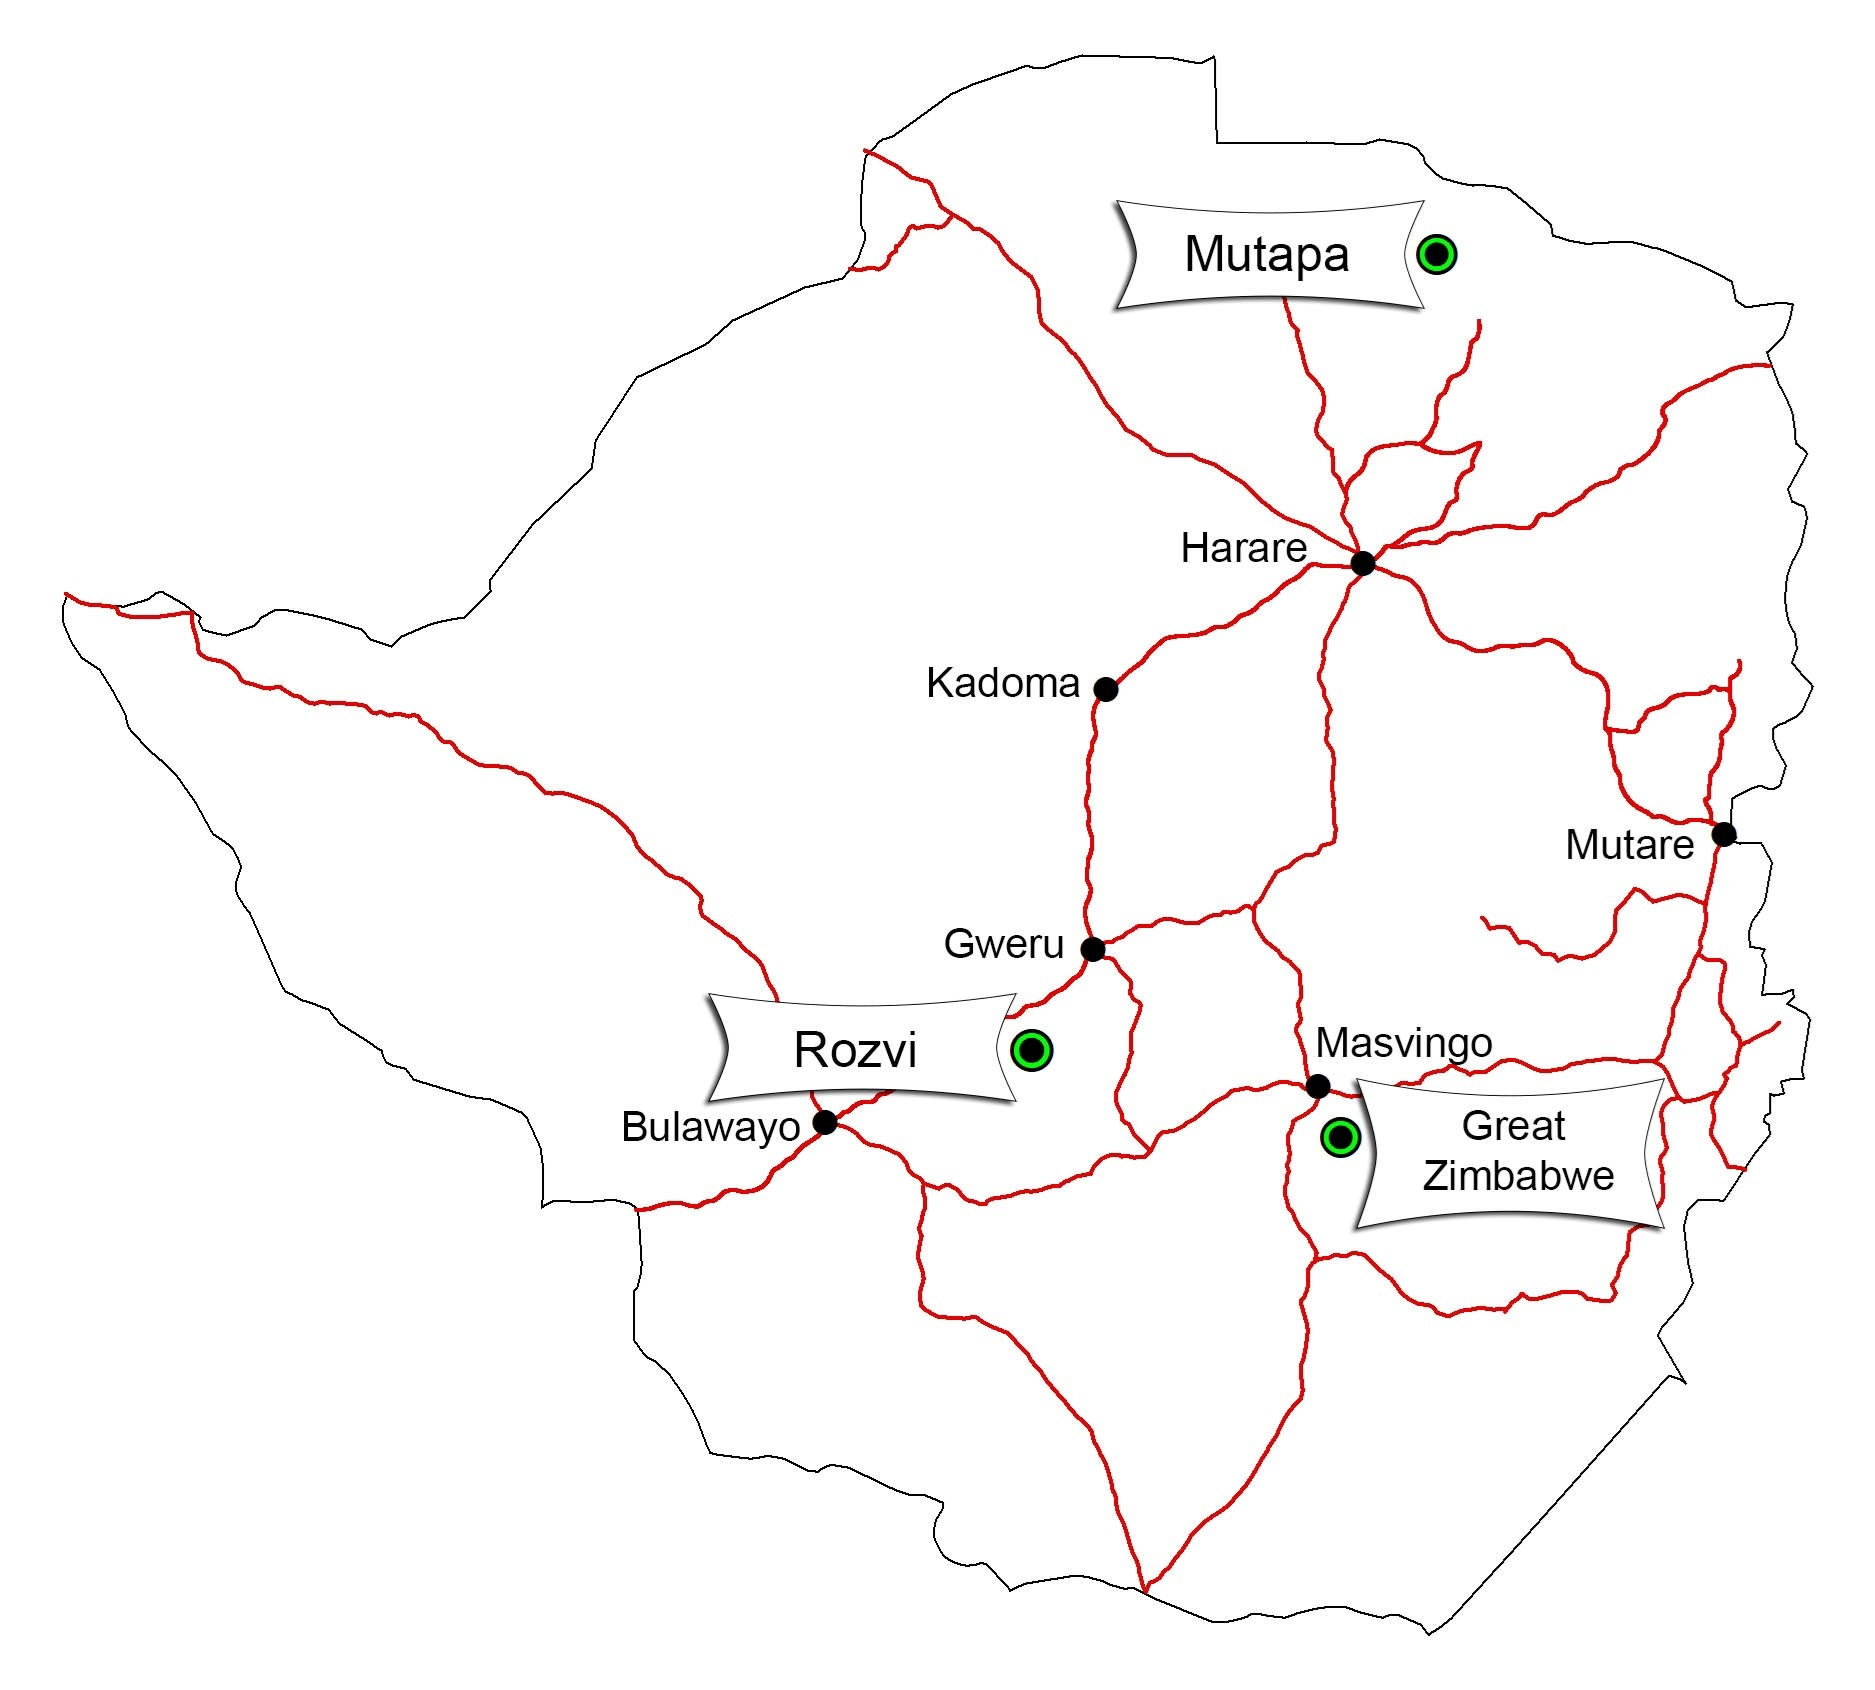
\includegraphics[width=\linewidth]{Nyambiya_Figure_01}
	\caption{Map showing Great Zimbabwe, Mutapa and Rozvi states
		{\normalfont\scriptsize \\ \copyright\ Rusell Kapumha. Permission by copyright owner.
	}
}
	\label{fig:Nyambiya_Figure_01}
\end{figure}

The second phase of the Zimbabwe Culture is Great Zimbabwe from 1250-1550 CE (\cites{pikirayi2006}{kim2008}). With regards to dry stone walling, the Zimbabwe Culture has mainly two types: terraced walls for platforms and freestanding walls for enclosures \parencite{chirikure2013socio}. The freestanding walls, decorated with a chevron pattern, housed the elite and characterize the Great Zimbabwe phase of the Zimbabwe Culture.

The third phase of the Zimbabwe Culture is Khami, which spans from 1450 to 1820 CE (\cites{manyanga2006}{chirikure2014}).  Khami was  part of the Torwa polity. In terms of pottery designs, Khami phase is characterized by bands and panels of black and red motifs (\cites{huffman2011}{chirikure2013socio}). In the Khami phase, freestanding walls are rare as the phase is dominated by terraced platforms decorated by a check pattern (\cites{huffman2011}{huffman2012}{chirikure2013socio}). This herringbone pattern represents chiefs residences (\cites{pikirayi2007}{huffman2011}).

Since regional and interregional trade networks are visible in the Zimbabwe Culture from Mapungubwe phase, the Farming Communities (formerly referred to as The Iron Age) experience was  profoundly transformative in the social, economic and political spheres of southern Zambezia \parencite{pikirayi2007}.
Zambezia refers to the regions drained by the Zambezi River and the Zimbabwe plateau (\cite[][3]{pikirayi2001}). It covers five countries namely Zambia, Zimbabwe, Botswana, South Africa, and Mozambique \parencite{kim2008}.
As early as 700 CE local networks of trade and exchange appear to be common, intensifying by 800 CE at Great Zimbabwe, and  reached their peak by 1200 CE \parencites{kusimba1999}{kim2008}.

The impact of both international and regional trade to past societies is crucial in the understanding of the organization of these societies. The investigation of the importance of trade to pre-colonial Zimbabwe and beyond illuminates aspects of economic, political, and social organization. Trade relations and exchange between the coast and pre-colonial Zimbabwe is traceable from 700 CE to 1700 CE \parencite{pwiti2005}. The scale of regional trade is not fully known and estimates suggest it was relatively small scale in the early phases; but by the 1200 CE,  long-distance exchange between the coast and inland southern Africa was well established (\cites{pwiti1991}{pwiti2005}{chiripanhura2017}). In most works, the effects of regional trade to past societies is undermined and overlooked, while that of international trade attracts more emphasis. Trade, be it regional or international, had profound effects to communities of Zimbabwe prior to its colonization.

The aim of this paper is two fold. First, it seeks to understand the role and effects of regional and interregional trade which involved pre-colonial Zimbabwean societies. Secondly, it is geared towards initiating reasearch on regional trade in southern Africa and interregional trade with other regions of the continent. In this paper, regional trade implies the contact of societies of the same region, in this case, societies of southern Africa. Interregional trade, on the other hand, implies contact of societies of different regions but of the same continent, for example trade between southern Africa and central Africa.

\IJSRAsection{Great Zimbabwe}

Following the demise of Mapungubwe in 1290 CE, dominance of trade routes shifted to Great Zimbabwe, which became a political, economic, and cultural sucessor to Mapungubwe (\cites{pikirayi1993}{pwiti2005}{manyanga2006}). Great Zimbabwe covered an area of 700 ha making it one of the largest states in Sub-Saharan Africa, built over centuries beginning 900 CE (\cites{sinclair1993}{ndoro1997}{ndoro2001}).
The impressive architecture is estimated to have had a population of around \num{20000} (\cites{garlake1973}{hall1990}{kim2008}). However, recent research on the population of Great Zimbabwe estimates 5000 inhabitants \parencite{chirikure2017}.
Great Zimbabwe has been a subject of debate for centuries with regards to its origins, known as the \enquote{Zimbabwe Controversy} \parencite{tangri1990},
but this debate has long been resolved to be \enquote{essentially African} in origin and character (\cites{randall1906}{ndoro1997}). Current debates on Great Zimbabwe revolve upon the use and interpretation of space
(see \cites{huffman1984a}{huffman1984b}{huffman1996}{huffman2010}{huffman2014}
on the other hand, \cites{beach1998}{chirikure2008}{pikirayi2011}{chirikure2013socio}).

Regional trade played a crucial role to the economy and social organization of pre-colonial societies within the Zimbabwe plateau. At Great Zimbabwe, iron gongs identical to those found in Zambia at Ingombe Ilede provide evidence of regional trade \parencite{garlake1973}. However, the small quantities of these items at Great Zimbabwe might suggest that these were gifts presented to the royalty rather than a trade item. Copper crosses and barbed spearheads were imports found at Great Zimbabwe from central Africa (\cites{pikirayi2006}{pikirayi2017}). Local products from Great Zimbabwe for regional and interregional trade included soapstone, gold wire, and perforated gold sheets (\cites{garlake1973}{pikirayi2006}{pikirayi2017}).

Great Zimbabwe’s regional trade links, led to the development of monumental architecture in Makgadikgadi Pans in Botswana \parencite{pikirayi2017}, such that local and interregional trade thrived and these iron-using farming communities prospered. From the \nth{14} century to the 15th century CE, metal and copper working was intensively and extensively traded by people from Great Zimbabwe \parencite{garlake1973} though it was mainly for regional and interregional trade. Hence, the importance of this branch of economy is not to be underestimated as the participation in international trade serves as a metaphor of  the efficiency of local economies through regional and interregional trade (\cites{pwiti1991}{pwiti2005}{manyanga2006}{pikirayi2006}).

The appearance of these trade goods in the interior of southern Africa particularly at Great Zimbabwe is explained by the trade role of  communities settled along the East African coast. Communities along the East African coast had established trade networks with traders from other continents prior to the \nth{13} century CE,
a period in which Great Zimbabwe became a major trading centre in southern Africa. When Great Zimbabwe emerged as a major trading centre, the communities along the east African coast still arbitrated the transoceanic trade. Goods were exchanged through intermediaries at Kilwa, Mafia, or Mogadishu but Arabs and Asians did not penetrate the interior of Africa \parencite{alradi1990}. Consequently, east African coastal centres became affluent from the taxes levied on goods leaving the coast \parencite{alradi1990} and for Kilwa, this is supported by the impressive monumental architecture like the Grand Palace of Husuni Kubwa \parencite{pikirayi2006}.
At Great Zimbabwe, a coin minted by al-Hasan ibn Sulaiman (1230--1233 CE), ruler from Kilwa was recovered showing the eminence of the east African coast centres in this viable trade interaction
\parencite{pikirayi2006}. By the \nth{12} century CE, Great Zimbabwe had extended its trade networks to the coast and to international trade, which became its major trading partner (\cites{pwiti2005}{kusimba2007}{kim2008}). This development was an important aspect of the economy of Great Zimbabwe, which however interlaced an already complex economy.

Great Zimbabwe prospered and reached its peak in the \nth{13} century CE, which is demonstrated by its unparalleled architecture within the region. Wealth from regional and interregional trade could finance the massive investment of dry stone architecture at Great Zimbabwe \parencite{kim2008}.
Great Zimbabwe was also involved in international trade which however, began to decline in the \nth{15} century CE. This is indicated by the rare appearance of Chinese porcelain at Great Zimbabwe as the porcelain was now traded elsewhere in the Zimbabwe plateau \parencite{pikirayi2006}.
Despite the strenghtened links between Great Zimbabwe and the coast, in the post \nth{15} century CE period, \enquote{Great Zimbabwe was no longer trading} internationally (\cite[][135]{garlake1973}). Thus, in southern Africa particularly at Great Zimbabwe, international trade was considerably short-lived compared to regional and interregional trade.

\IJSRAsection{Mutapa state}
Little is known archaeologically about the Mutapa state and much of the literature available is historical, thus, attracting more historians than any other kind of researchers \parencite{pikirayi1993}.
The Mutapa state was confined to the north of the Zimbabwean plateau occupying areas between Zambezi river to the north, Hunyani river to the southwest, and Mazoe river to the southeast (\cite[][1]{beach1976}).
The rise and development of the Mutapa state is linked to the demise of Great Zimbabwe, after people migrated from the southern part of the Zimbabwean plateau to the northern part, where developments took place from 1450-1900 CE \parencite{pikirayi2006}.

There are suggestions that these migrations were caused by the deterioration of the environment leading to the demise of Great Zimbabwe \parencite{huffman1972}. However, recent research has established that Great Zimbabwe declined at a time when environmental conditions were favourable (\cites{pikirayi2001}{pikirayi2006}{pikirayi2017}{chirikure2017}).
The development of these historical states, such as Mutapa, rose as populations considered other areas to settle including the availability of resources for exploitation. Traditions on the establishment of the Mutapa state centres on the myth that the inhabitants of Great Zimbabwe left the southern part of the Zimbabwean plateau to the north in search of salt \parencite{ab1961}.
This implies two critical observations to this discussion of trade, shifting trade routes and the impact of trade to pre-colonial Zimbabwean societies:
there is an indication of diminution of resources at Great Zimbabwe causing a shift in dominace of trade.

Trade, both regional and international, was essential to the economy of the Mutapa state. As a means of consolidating their power and authority, the leaders of the Mutapa state controlled economic activities but did not monopolize it
\parencites{mudenge1974}{mudenge1988}.
With local trade, the leaders of the Mutapa state depended on the alacrity of their subjects \parencite{chanaiwa1972}.
On international trade, the leaders of the Mutapa state relied on tax levied on exports and imports. The northern part of Zimbabwe (where the Mutapa state was located) was rich in gold, silver, ivory, and copper which was destined for regional and international markets
\parencite{chanaiwa1972}. The Mutapa state exported these natural resources in exchange for manufactured products, such as cloth and beads. The exploitation of these natural resources was permitted only by the Mwene Mutapa, who was the king of the Mutapa state. The Mwene Mutapa owned royal mines that locals, fellow inhabitants of the Mutapa state worked in and were rewarded by cattle \parencite{chanaiwa1972}. Once the natural resources were obtained, the locals would trade with the Portuguese. It is key to note that the Mutapa state was one of the main contributors of interregional trade through gold, copper, ivory,
and cattle (\cite[][126]{kusimba1999}).

However, from the 17\textsuperscript{th} century CE,
civil wars and local rivalries were exacerbated by Portuguese intervention which destabilized African societies (\cites{chanaiwa1972}{alradi1990}{kinahan2000}).
The Portuguese affected not only the economy of the Mutapa state but the politics of this state, as the Portuguese were agents of disintegration of the complex Mutapa state (\cite[][435]{chanaiwa1972}).
In the 17\textsuperscript{th} century CE, the Mwene Mutapa became very unpopular and his power dwindled drastically. Consequently, he was incapable of consolidating the peace and order necessary for the success and flourishing of trade; hence, trade was interrupted \parencite{chanaiwa1972}.
In summary, as stated by \textcite[][435]{chanaiwa1972}, \enquote{the economy was gone}.

\IJSRAsection{Rozvi state}

The Rozvi state emerged after the decline of Great Zimbabwe, this is likely due to shifting trade routes in mid 15\textsuperscript{th} century CE. The Rozvi state is dated between 1450 and 1830 CE \parencite{pikirayi2006}. This historic state has not attracted much archaeological attention, but rather historical like the Mutapa state. The Rozvi state was a political successor of the Torwa state which had its capital at Khami
(\cites{pikirayi2006}{pikirayi2013hist}{manyanga2010}). The Rozvi state was founded by a Changamire, the Rozvi king, who in 1670 CE stormed and captured the Torwa. This led to the formation of the Rozvi state, with its capital at Danamombe in south-western Zimbabwe (\cites{mudenge1988}{beach1980}[][17]{huffman1996}). The Rozvi state mainly traded with the Portuguese.

From the archaeological record and historical accounts, the Rozvi craftsmen worked iron, copper, bronze, and gold, produced carved objects  from ivory and soapstone, and made beads from ostrich egg shells \parencite{mudenge1974}.
From soft metals, the Rozvi made bangles, chains, earrings, and bracelets. These products ensured that the economy of the Rozvi state flourished through interregional trade. Since agriculture and pastoralism were the basis of the economy of the Rozvi state \parencite{mudenge1974}, cattle was the main export destined for regional trade. However, this trade item (cattle) is very problematic to prove from the archaeological record. For \textcite{mudenge1974}, cattle was the economic prop of the Rozvi state.

\IJSRAsection{Discussion}
After discussing the economic organization of the main clusters of pre-colonial Zimbabwe, I  look at international trade involving these societies. Furthermore, the implication of regional and interregional trade to international trade will also be discussed.

Global trade from around 1200 CE diversified the economy and society of Great Zimbabwe.  Among the principal exports from the region were gold and ivory (\cites{mudenge1988}{pwiti2005}{pikirayi2006}). The imports included cowrie shells, porcelain, celadon, Far and Near Eastern stoneware (\cites{garlake1973}{garlake1982}{pikirayi2006}), glazed Persian bowls with inscription of Naskhi characters dated to the 13\textsuperscript{th} or 14\textsuperscript{th} century CE (\cites{garlake1973}). Among the imports were glass beads of various colours of an Indian and Persian origin (fig 2) and Islamic wares (\cites{huffman1972}{huffman2000}{kim2008}{chirikure2008}). The imported glass beads recovered from Great Zimbabwe (fig 2) are identical to those found at centres of the East African coast (\cites{chirikure2008}{kusimba2017}). It is probable that the appearance of exotic goods in the interior of southern
Africa was the work of Arab and later Swahili traders (\cites{kusimba1999}[][22]{ndoro2001}).
Therefore, the earliest international contact with pre-colonial Zimbabwe societies was with the Eastern world. As a result of the colonial contact, European goods found their way into southern Africa during the 15\textsuperscript{th} century CE.

%FIGURE 02: Beads
\begin{figure}[!tb]
	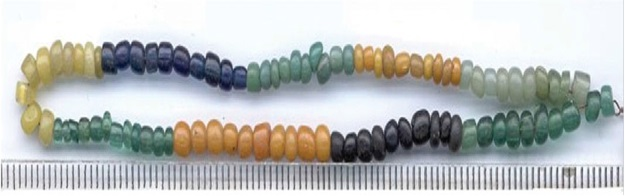
\includegraphics[width=\linewidth]{Nyambiya_Figure_02}
	\caption{Example of imported glass beads found at Great Zimbabwe
		{\normalfont\scriptsize \\ \copyright\ Marilee Wood
	}}
	\label{fig:Nyambiya_Figure_02}
\end{figure}
%image permission?

During the  Mutapa phase the Portuguese, centered in coastal Mozambique, became the main trading partners. The Portuguese were more interested in monopolizing extractive economies, especially gold from the Mutapa state.
After the 1500 CE, the Portuguese aimed at trading directly with African societies including the Mutapa state. Consequently, trading markets (\emph{feiras}) were established at places such as Dambarare, Manyika and Rimuka \parencites{Pikirayi1993,Pikirayi2009}.
By so doing, the Portuguese aggressively sought to overthrow Swahili and Arab traders of the east African coast, who had pioneered these networks of
exchange (\cites{sinclair1987}{kusimba1999}{pwiti2005}).

The Rozvi \emph{mambo}, (King of the Rozvi state) by allowing individual participation in long-distance trade avoided rousing undue resentment, but his wealth from external trade was through tribute. Tribute was paid in form of gold, ivory, beads, and cloth, which were the main returns of external trade \parencite{mudenge1974}. It is in this regard that tribute was important to the leaders of the Rozvi state as it served dual purpose: economic and political.
From the Portuguese, the Rozvi received luxury goods like beads, seashells, brass bells, and cloth \parencite{mudenge1974}.
Imports from other continents beyond Africa were important even to the consolidation of power and authority in the Rozvi state. One example is of imported cloth which played an important role in the politics of the Rozvi state. At the investiture of a new chief, the Rozvi mambo would send black and white calico as the official regalia of the new chief (\cites{mudenge1974}{bvocho2005}).
Giving the new chief black and white calico might imply the rarity of the cloth. If, however,  the cloth was abundant, possibly there was no need to send it to the new chief as the chief could easily acquire the regalia. Or, it may also imply that the cloth was in abundance, but as a sign of the mambo’s recognition of the new chief, he would send the imported cloth
\parencite{bvocho2005}. It seems more likely that the latter was the situation since long-distance trade in the Rozvi state was open to individual participation. Nonetheless, the imports within the Rozvi state were luxury goods, which had other internal valuable alternatives
\parencite{mudenge1974}.

The evidence of international trade involving pre-colonial Zimbabwe attests to the presence of regional and interregional trade. From the interior of southern Africa, trade items for international trade had to pass through the east African coast \parencite{pwiti2005}. The towns of Zuama and Angoche on the Zambezi Delta, for example, were centres where gold and ivory from the Mutapa state was exchanged for cotton, silk, and beads (Barbosa, 1917:15 as cited in \cite[][130]{kusimba1999}). During international trade, east African coastal centres played an intermediary role linking southern Africa and regions beyond. Trade goods from the interior of Africa were transported to coastal centres like Sofala and Kilwa which was the primary beneficiary of the gold trade from Zimbabwe (\cites{miller2000}{pwiti2005}{pikirayi2006}{huffman2009}).
As a result of the prosperity of this gold trade in the 13th century CE mirrored also at Kilwa, the Grand Palace of Husuni Kubwa reflects the wealth of this state system (\cites{pikirayi2006}{pikirayi2017}).
As noted by \textcite[][387]{pwiti2005} and \textcite{pikirayi2017},
communities at Kilwa and in pre-colonial Zimbabwe benefited from each other.

Once these goods reached these trading centres, traders from other continents were not allowed into the interior of Africa \parencite{alradi1990}. In light of the above, \textcite{kusimba1999} and \textcite{manyanga2006} note that the implication of regional and interregional trade to international trade is that the former required great planning and organization without which the latter could not be established. Hence, from the nature of the organization of international trade, it seems most probable that regions in Africa were involved in trade with each other. In support of this, \textcite{pwiti2005} notes that the decline of Great Zimbabwe in the last half of the 15th century CE is associated with the same development at Kilwa. Thus, the emerging economic picture between these states is that of a symbiotic relationship.

\IJSRAsection{Regional and interregional trade involving Zimbabwe: Future prospects}
After discussing the evidence of regional and interregional trade, I will now discuss possible methods that researchers may employ in order to address pre-colonial regional and interregional trade. The application of the methods discussed was drawn from regions where they have been used elsewhere but are still lagging behind in Zimbabwean archaeology. The few methods given here are, however, for purpose of illustration. From the available literature, there is overwhelming evidence of international trade involving southern African societies.  This might be a result of the role of international trade, which early researchers assumed was the prime mover in the development of socially complex societies (\cites{huffman1972}{huffman1982}{huffman1986}{huffman2009}). %how to format multi-year?
However, very little is known about regional and interregional trade. Thus, the methods discussed here, if employed, are aimed at increasing our knowledge of pre-colonial regional and interregional trade, which involved pre-colonial Zimbabwe.

The ubiquity of glass beads recovered in southern Zambezia beginning from the Mapungubwe phase have provided the finest example of interregional networks.  Due to their portability, affordability, and durability, glass beads were consumed over much of the region and provide the finest signature for evaluating the nature, scale, and distribution of interregional trade \parencite{dussubieux2008}.  Advances in geochemistry have made it possible to carry out relatively cheap composition analyses of glass beads.  For example, X-Ray Fluorescence (Wavelength Dispersive XRF and portable XRF) is a non-destructive technique that is used to characterise major and minor elements of glass to enable the determination of the overall mineralogical and elemental signature of the samples (\cite[][245]{pernicka2014}). These techniques have been used to source the origins of this trade item, as their sources can be established \parencite{wood2000}. In a recent study of glass beads produced between 800 and 1600 CE, Robertshaw and colleagues established that Zhizo beads dating between the 8th and 10th century CE were made from plant-ash, which is specific to the Middle East, probably Iran and not from South Asia as had been previously assumed \parencite{robertshaw2010}.

Important evidence on the investigation of this topic on pre-colonial Zimbabwean societies is metals, which were exchanged for livestock and grain. Some iron products were hoes, axes, and spear heads. While gold, ivory, and other valuables were destined for international consumption, iron and copper provide evidence for regional trading networks (\cite[13]{pikirayi2017}). Metals in southern Africa were influential in determining regional trade as metallurgy led to opportunities for trade and exchange at local, regional, and international scales (\cites{chirikure2007}{chirikure2013post}). On archaeometallurgical research in Zimbabwe, the work of
\citeauthor{chirikure2005}
\parentext{%
\citeyear{chirikure2005},
\citeyear{chirikure2006},
\citeyear{chirikure2007},
\citeyear{chirikure2010},
\citeyear{chirikure2015}}
has been exceptional in the last decade or so. Nonetheless, \textcite[][152]{chirikure2013post} acknowledge that archaeometallurgy in Zimbabwe is still in its infancy. This has been a major setback to the overall appreciation of ancient metals.
For example, ingots (known as Katanga crosses) have been found at Great Zimbabwe and their presence has been used as evidence of trade between Great Zimbabwe and central Africa. To date, no geochemical work has been carried out to prove that Katanga is the source of such items.

Similarly, archaeometallurgical studies based on chemical elemental and lead isotopic composition have been instrumental in the analysis of ancient metal working. Lead has four isotopes that are stable,
these are
\textsuperscript{206}Pb,
\textsuperscript{207}Pb,
\textsuperscript{208}Pb and
\textsuperscript{204}Pb.
The first three are time dependent and are produced by the radioactive decay of parent isotopes
\textsuperscript{238}U,
\textsuperscript{235}U and
\textsuperscript{232}Th, respectively.
\textsuperscript{204}Pb is stable but time independent as its abundance has not changed from the formation of the earth (\cites{molofsky2009}{baron2014}{pernicka2014}). The application of lead isotopic analyses in archaeology is based on the premise that sources of metals can be distinguished from each other. For example, deposit on bivariate plots (e.g.,
\textsuperscript{208}Pb/\textsuperscript{204}Pb vs \textsuperscript{207}Pb/\textsuperscript{204}Pb) gives a unique signature for that deposit which is used to match its parent ore source \parencite{molofsky2009}. \textcite{molofsky2009} employed metal provenance studies in southern Africa to understand metal objects from this region. They established that Rooiberg was the source of tin and soft metal working in southern Africa.

Evidence of regional and interregional trade in southern Africa and beyond is also in the form of ceramics.
As evidence of trade, \textcite[][22]{garlake1968} observes that prior to the dominance of Portuguese as the major trading partner with Africa, over \SI{90}{\percent} of imported ceramics found in central Africa were from Zimbabwe. Thus, ceramics were used in trade relations that were essential to the economy of pre-colonial Zimbabwean societies. Regardless of the centrality of ceramics to past societies, there still remains a handful archaeometric research to understand the role of ceramics in the discusion of trade and exchange in Zimbabwean archaeology  (\cites{lindahl2010}{ashley2015}).

The application of petrographic analysis and ceramic provenance studies is vital in the appreciation of trade and exchange of ceramics. Ceramics survive long in the archaeological record, hence, the increased potential to subject this material to a wide range of analyses. In most Zimbabwean archaeological studies, ceramics have been used as pointers to culture change, identify traditions, and patterns of migrations (\cites{huffman1972}{pikirayi1993}{pikirayi1996}{pwiti1996}) without necessarily looking at how this material culture could have been used in trade and exchange regionally. \textcite{wilmsen2009} used petrology and clay chemistry to identify the origins of ceramics from Botswana. Their study showed that most of the clay constituents were from Angola, thus, showing patterns of trade and exchange through ceramics.

Overall, tradtional archaeology complemented by laboratory studies clearly demonstrate that networks of exchnage in Africa were vast. The scale of production and investment in local extractive economies including mining, smelting, and making metallurgical products including gold, tin, and iron for wide distribution was well established by 1200\CE.

\IJSRAsection{Conclusion}
Contacts involving pre-colonial Zimbabwean societies resulted in an exchange of goods and ideas \parencite{pikirayi2017}. Such contacts have often been viewed in international perspective as the main consolidator of wealth \parencite{manyanga2006} and a precursor of power \parencite{kusimba2017} thereby limiting the appreciation of regional and interregional contacts. However, regional and interregional trade was an important facet in the economies of the societies under study, that is the Great Zimbabwe, Mutapa, and Rozvi states. The complexity of interregional trading systems involving southern Africa indicates that interregional trade within Africa was the foundation on which international trade was based. As such, the participation of pre-colonial Zimbabwean societies in international trade indicates the thriving of regional and interregional trade.

 Several spheres of exchange including long distance international, regional and interregional interactions characterise pre-colonial Zimbabwean societies. These spheres of exchange transcended state boundaries within and across continents.
In spite of this, archeaological research in southern Africa, particularly Zimbabwe, to understand regional and interregional trade is still minimal. The application of characterisation studies in the study of archaeological artifacts will advance our knowledge of the evolution of the states in southern Zambezia. Particularly for Zimbabwean archaeology, complementary techniques drawn from geochemistry, and metallurgy will transform our understanding of pre-colonial Zimbabwean economies. There is need for Zimbabwean archaeology to fully embrace the aspirations of the New Archaeology. Thus, there is a bright future for Zimbabwean archaeology to explore pre-colonial regional and interregional trade.



\IJSRAsection{Dedication}
To my loving parents Clement Nyambiya and Rubbee Mutanda-Nyambiya.

\IJSRAsection{Acknowledgements}
I thank Ancila Nhamo, Chapurukha M. Kusimba,
Alba Menendez Pereda and Munyaradzi Elton Sagiya who shared their useful insights to this manuscript.
I am grateful to Rusell Kapumha who produced the map in this paper (\cref{fig:Nyambiya_Figure_01}).
I also thank The Mirror International Research Institute (TMIRI) for funding my stay in Tanzania.

\IJSRAclosing%<---- don’t change this!
